\input{./preambule-2010-utf8.ltx}


\ifdefined\COMPLETE
\else
    \newcommand{\COMPLETE}
\fi                        % Autorise la compilation de illustrations
                          % soit isolées, soit inluses 

\ifdefined\CORRECTION
\else
    \newcommand{\CORRECTION}
\fi                        

\begin{document}

\newcommand{\chapitre}[1]{{\bf #1}\medskip
}

\chapitre{Chapitre 1}
       \ifdefined\COMPLETE
\else
    \input{./preambule-2010-utf8.ltx}
    \begin{document}
\fi

\ifdefined\CORRECTION
    \begin{alterqcm}[lq=11cm,correction]
\else
    \begin{alterqcm}[lq=11cm]
\fi

 \AQquestion[br=2]{Une expression développée est\ldots}{%
 {$(x-1)(x+2)$,},
 {$x^2+x-2$,},
 {$x(x-1)+2x-2$.}
 }



\AQquestion[br=3]{Le développement de $(a+b)^2$ est\ldots}{%
 {$a^2+b^2$,},
 {$a^2+ab+b^2$,},
 {$a^2+2ab+b^2$.}
 }

\AQquestion[br=3]{Le développement de $(a-b)^2$ est\ldots}{%
 {$a^2-b^2$,},
 {$a^2+2ab-b^2$,},
 {$a^2-2ab+b^2$.}
}

\AQquestion[br=1]{Le développement de $(a-b)(a+b)$ est\ldots}{%
 {$a^2-b^2$,},
 {$a^2+b^2$,},
 {$a^2-2ab+b^2$.}
}

\AQquestion[br=2]{Une expression factorisée est\ldots}{%
{$(x-2)^2+(x-2)(x-1)$,},
{$(x-2)(2x-3)$,},
{$2x^2-7x+6$.}
}


\AQquestion[br=1]{$A = (x-1)(x+2)-5(x-1)$}{
{\begin{minipage}[t]{6cm}
   l'expression $A$ peut être factorisée \\
   avec un facteur commun évident,
\end{minipage}},
{\begin{minipage}[t]{6cm}
   l'expression $A$ peut être factorisée \\
   avec une identité remarquable, 
\end{minipage}},
{\begin{minipage}[t]{6cm}
   l'expression $A$ \\ 
   ne peut pas  être factorisée.
\end{minipage}}
}


\AQquestion[br=2]{$A = 9x^2 -2x + \dfrac{1}{9}$}{%
{\begin{minipage}[t]{6cm}
   l'expression $A$ peut être factorisée \\
   avec un facteur commun évident,
\end{minipage}},
{\begin{minipage}[t]{6cm}
   l'expression $A$ peut être factorisée \\
   avec une identité remarquable, 
\end{minipage}},
{\begin{minipage}[t]{6cm}
   l'expression $A$ \\ 
   ne peut pas  être factorisée.
\end{minipage}}
}

\end{alterqcm}

\ifdefined\COMPLETE
\else
    \end{document}
\fi      
\newpage

\chapitre{Chapitre 2}
       \ifdefined\COMPLETE
\else
    \input{./preambule-2010-utf8.ltx}
    \usepackage{alterqcm}
    \begin{document}
\fi

\ifdefined\CORRECTION
    \begin{alterqcm}[lq=9cm,correction]
\else
    \begin{alterqcm}[lq=9cm]
\fi



 \AQquestion[br=2]{Pour résoudre l'équation $1-3x=8x+5$,\\
 on peut se ramener à la résolution de l'équation\ldots}{%
 {$-11x = -4$,},
 {$11x = -4$,},
 {$5x=6$.}
 }
 

 \AQquestion[br=2]{Pour résoudre l'équation $ (2x-1)(2-3x)=0$,\\
  on peut se ramener à la résolution de l'équation\ldots}{%
 { on développe $(2x-1)(2-3x)=0$, },%
 {\begin{minipage}[t]{8cm} on résout chacune des équations \\
        $2x-1=0$ et $2-3x=0$,
    \end{minipage}},%
   {\begin{minipage}[t]{8cm} on divise chaque membre de l'équation par $2-3x$.
  \end{minipage}}
 }
 
 
 \AQquestion[br=3]{Si $b>c$, alors\ldots}{%
   {\begin{minipage}[t]{6.5cm} on ne peut pas comparer $-2b$ et $-2c$, \end{minipage}},
 {$-2b > -2c$,},
 {$-2b < -2c$.}
 }
 
  
 \AQquestion[br=1]{Les solutions de l'inéquation $-2x \geqslant 4$}{%
    {\hbox {\raise -4.5mm \hbox{\begin{tikzpicture}[scale=.65]
         \tkzInit[xmin=-5,xmax=4,xstep=1]
         \tkzDrawX
         \tkzXHW     {-5/F//-2/T/] } % Hachures de -inf à -2
         \tkzText(0,-.6){\scriptsize $0$}  
         \tkzText(-2,-.6){\scriptsize $-2$}  
      \end{tikzpicture} }              
     }},
    {\hbox {\raise -4.5mm \hbox{ \begin{tikzpicture}[scale=.65]
         \tkzInit[xmin=-5,xmax=4,xstep=1]
         \tkzDrawX
         \tkzXHW     {-2/F/[/4/ } % Hachures de -inf à -2
         \tkzText(0,-.6){\scriptsize $0$}  
         \tkzText(-2,-.6){\scriptsize $-2$}  
      \end{tikzpicture}
    }}},                
    {\hbox {\raise -4.5mm \hbox{ \begin{tikzpicture}[scale=.65]
         \tkzInit[xmin=2,xmax=10,xstep=1]
         \tkzDrawX
         \tkzXHW     {6/F/[/10/ } % Hachures de -inf à -2
         \tkzText(2,-.6){\scriptsize $2$}  
         \tkzText(3,-.6){\scriptsize $3$}  
         \tkzText(6,-.6){\scriptsize $6$}  
      \end{tikzpicture}                 
     }}}
 }
 
 \AQquestion[br=3]{Les solutions de l'inéquation $-3x \geqslant 0$, sont les nombres\ldots}{%
   {$x \geqslant 0$,},
 {$x \geqslant 3$,},
 {$x \leqslant 0$.}
 }


 \AQquestion[br=3]{Pour résoudre l'équation $2-5x>-2x+1$,
 on peut se ramener à la résolution de l'équation\ldots}{%
 {$1>-7x$,},
 {$-3x<1$,},
 {$3x<1$.}
 }


 \AQquestion[br=1]{« Julie a 15 ans et son père a 42 ans. Dans combien d'années l'âge de son père sera égal au double de l'âge de Julie ? » \\
 Pour résoudre ce problème, il faut commencer par}{%
 {préciser l'inconnue choisie,},
 {écrire une équation,},
 {résoudre une équation.}
 }
 
\end{alterqcm}

\ifdefined\COMPLETE
\else
    \end{document}
\fi
\newpage

\chapitre{Chapitre 3}
       \ifdefined\COMPLETE
\else
    \input{./preambule-2010-utf8.ltx}
    \begin{document}
\fi

\begin{alterqcm}[lq=8cm]



 \AQquestion[br=2]{On ne peut calculer la racine carrée d'un nombre $a$ que si\ldots}
  {%
   {$a$ est un nombre entier},
   {$a \geqslant 0$},
   {$a \leqslant 0$}
 }

 \AQquestion[br=1]{Si $a$ désigne un nombre positif, alors $\sqrt{a}$ désigne\ldots}{%
   {le nombre positif dont le carré est $a$},
   {la moitié de $a$},
   {le carré de $a$}
 }
 

 \AQquestion[br=2]{Si $a$ désigne un nombre positif, alors $\sqrt{a^2}$ est égal à \ldots}{%
   {$\dfrac{1}{2} a$},
   {$a$},
   {$\dfrac{1}{2} a^2$}
 } 

 \AQquestion[br=3]{L'équation $x^2 = 5$\ldots}{%
   {n'a pas de solution,},
   {a une seule solution},
   {a deux solutions opposées}
 } 


 \AQquestion[br=1]{L'équation $2x^2 +3 = 0$\ldots}{%
   {n'a pas de solution,},
   {a une seule solution},
   {a deux solutions opposées}
 } 


 \AQquestion[br=2]{$\sqrt{2} \times \sqrt{3}$ est égal à \ldots}{%
   {$\sqrt{5}$},
   {$\sqrt{6}$},
   {6}
 } 


 \AQquestion[br=1]{$\sqrt{\dfrac{5}{3}}$ est égal à \ldots}{%
   {$\dfrac{\sqrt{5}}{\sqrt{3}}$},
   {$\dfrac{\sqrt{5}}{3}$},
   {$\sqrt{2}$}
 } 

 \AQquestion[br=1]{$\dfrac{2}{\sqrt{2}}$ est égal à \ldots}{%
   {$\sqrt{2}$},
   {$2\sqrt{2}$},
   {$\dfrac{\sqrt{2}}{2}$}
 }  
 

 \AQquestion[br=3]{$\sqrt{72}$ peut s'écrire \ldots}{%
   {$36\sqrt{2}$},
   {$2\sqrt{6}$},
   {$6\sqrt{2}$}
 }  
 
 \AQquestion[br=2]{$3\sqrt{20} - \sqrt{45}  \sqrt{5}$ peut s'écrire sous la forme\ldots}{%
   {$a\sqrt{3}$ avec $a$ nombre entier,},
    {$a\sqrt{5}$ avec $a$ nombre entier,},
   {$a\sqrt{2} + b\sqrt{5}$ avec $a$ et $b$ nombres entiers}
 }  
 
  
\end{alterqcm}

\ifdefined\COMPLETE
\else
    \end{document}
\fi
\newpage

\chapitre{Chapitre 4}
       \ifdefined\COMPLETE
\else
    \input{./preambule-2010-utf8.ltx}
    \begin{document}
\fi

\ifdefined\CORRECTION
    \begin{alterqcm}[lq=10cm,correction]
\else
    \begin{alterqcm}[lq=10cm]
\fi

 \AQquestion[br=1]{$\left(\sqrt{2}\right)^2$, est un nombre \ldots}{%
 {entier,},
 {décimal non entier},
 {irrationnel}
 }
 

 \AQquestion[br=1]{$\dfrac{3}{4}$, est un nombre \ldots}{%
 {entier,},
 {décimal non entier},
 {irrationnel}
 }

 \AQquestion[br=2]{$\dfrac{7}{3}$, est un nombre \ldots}{%
 {entier,},
 {décimal non entier},
 {irrationnel}
 } 
 

 \AQquestion[br=3]{$\left(1+\sqrt{2}\right)^2$, est un nombre \ldots}{%
 {entier,},
 {décimal non entier},
 {irrationnel}
 }


 \AQquestion[br=2]{36 admet\ldots}{%
 {six diviseurs,},
 {un seul diviseur,},
 {douze diviseurs}
 }
  

 \AQquestion[br=2]{Le {\sc pgcd} de 24 et 36 est\ldots}{%
 {4,},
 {12,},
 {24}
 }  

 \AQquestion[br=3]{L'algorithme d'{\sc Euclide} permet de calculer\ldots}{%
   {\begin{minipage}[t]{6cm}le plus petit diviseur commun à deux nombres,\end{minipage}},
   {\begin{minipage}[t]{6cm} le reste de la division euclidienne de deux nombres,
    \end{minipage}},
   {\begin{minipage}[t]{6cm} le {\sc pgcd} de deux nombres
    \end{minipage}}
 }
 
\AQquestion[br=2]{Deux nombres premiers entre eux\ldots}{%
   {\begin{minipage}[t]{7cm}n'ont aucun diviseur commun\end{minipage}},
   {\begin{minipage}[t]{7cm} admettent 1 pour seul diviseur commun,
    \end{minipage}},
   {\begin{minipage}[t]{7cm} sont deux nombres dontl'un est multiple de l'autre.
    \end{minipage}}
 } 
 

\AQquestion[br=3]{Une fraction irréductible est\ldots}{%
 {$\dfrac{45}{21}$},
 {$\dfrac{4220}{542}$},
 {$\dfrac{17}{14}$}
 }   

 
\AQquestion[br=2]{Pour rendre irréductible une fraction\ldots}{%
   {\begin{minipage}[t]{7cm}on soustrait de dénominateur au numérateur\end{minipage}},
   {\begin{minipage}[t]{7cm} on divise numérateur et dénominateur par leur {\sc pgcd},
    \end{minipage}},
   {\begin{minipage}[t]{7cm} on divise numérateur et dénominateur par un nombre quelconque, autre que 0.
    \end{minipage}}
 } 
\end{alterqcm}

\ifdefined\COMPLETE
\else
    \end{document}
\fi
\newpage

\chapitre{Chapitre 5}
       \ifdefined\COMPLETE
\else
    \input{./preambule-2010-utf8.ltx}
    \begin{document}
\fi

\thispagestyle{empty}
\vspace*{-2mm}

\ifdefined\CORRECTION
    \begin{alterqcm}[lq=10cm,correction]
\else
    \begin{alterqcm}[lq=10cm]
\fi


 \AQquestion[br=3]{Pour calculer l'image d'un nombre $x$ par la fonction linéaire de coefficient 4\ldots}{%
 {on additionne 4 à $x$},
 {on divise $x$ par 4},
 {on multiplie $x$ par 4}
 }
 

 \AQquestion[br=1]{$f$ est une fonction linéaire.\\
 l'écriture $f(2)=\dfrac{5}{4}$ signifie\ldots}
  {%
   {\begin{minipage}[t]{6cm} l'image de 2 par $f$ est $\dfrac{5}{4}$, \end{minipage}},
   {\begin{minipage}[t]{6cm} l'image de $\dfrac{5}{4}$ par $f$ est 2,\end{minipage}},
   {\begin{minipage}[t]{6cm} $f$ multiplié par 2 est égal à $\dfrac{5}{4}$.
    \end{minipage}}
 }

 \AQquestion[br=3]{Les prix augmentent de 2,5\%. Si $x$ désigne le prix initial et $f(x)$ le prix après l'augmentation, alors $f$\ldots}
  {%
   {\begin{minipage}[t]{7cm} n'est pas une fonction linéaire, \end{minipage}},
   {\begin{minipage}[t]{7cm} est la fonction linéaire de coefficient $\dfrac{2,5}{100}$,\end{minipage}},
   {\begin{minipage}[t]{7cm} est la fonction linéaire de coefficient $1,025$.
    \end{minipage}}
 }

 \AQquestion[br=1]{On note $V(x)$ le volume d'un cylindre de rayon $x$ et de hauteur 2 cm. La fonction $V$\ldots}
  {%
   {\begin{minipage}[t]{7cm} n'est pas une fonction linéaire, \end{minipage}},
   {\begin{minipage}[t]{7cm} est la fonction linéaire de coefficient 4,\end{minipage}},
   {\begin{minipage}[t]{7cm} est la fonction linéaire de coefficient $4\pi$.
    \end{minipage}}
 }

 \AQquestion[br=2]{Dans un repère, la représentation graphique d'une fonction linéaire\ldots}
  {%
   {\begin{minipage}[t]{8cm} est une droite quelconque, \end{minipage}},
   {\begin{minipage}[t]{8cm} est une droite qui passe par l'origine du repère,\end{minipage}},
   {\begin{minipage}[t]{7cm} est un segment de droite.
    \end{minipage}}
 }

 \AQquestion[br=1]{Dans un repère, la représentation graphique de la fonction linéaire de coefficient $a$ passe le point de coordonnées\ldots}
  {%
   {$(1;a)$},
    {$(a;1)$},
    {$(a;a)$}
 }



 \AQquestion[br=3]{Cette droite représente une fonction 
 \hspace*{1cm}\hbox{\raise -1.3cm \hbox {\begin{tikzpicture}[line cap=round,line join=round,>=triangle 45,x=5mm,y=5mm,scale=.7]
\draw [color={gray!40},dash pattern=on 1pt off 1pt, xstep=5mm,ystep=5mm] (-2.5,-2.5) grid (2.5,2.5);
\draw[->,color=black] (-2.5,0) -- (2.5,0);
\foreach \x in {-1,1}
\draw[shift={(\x,0)},color=black] (0pt,2pt) -- (0pt,-2pt);
\draw[->,color=black] (0,-2.5) -- (0,2.5);
\foreach \y in {-1,1}
\draw[shift={(0,\y)},color=black] (2pt,0pt) -- (-2pt,0pt) ;
\draw[color=black] (2pt,-7pt) node[left] {\footnotesize $0$};
\draw [red] (-2,2) -- (2,-2) ; 
\end{tikzpicture}}}\\
 \vspace*{-1.1cm} linéaire de coefficient\ldots, \\
 }
  {%
   {$a>0$},
    {$a=0$},
    {$a<0$}
 }
 
  \AQquestion[br=2]{Par la fonction ci-dessus, limage de -2\ldots}{%
   {se lit sur l'zxe des abscisses,},
    {se lit sur l'zxe des ordonnées,},
    {ne peut pas se lire.}
 }
 
  
  \AQquestion[br=2]{On dessine un rectangle $ABCD$ en diminuant de 20\% la longueur de chaque côté.\\
  Le dessin obtenu est une réduction de $ABCD$ dans un rapport\ldots}{%
   {0,2},
    {0,8},
    {1,2.}
 }
 
  
  \AQquestion[br=2]{On agrandit un prisme droit dans le rapport $\sqrt{}3$.\\
Son aire latérale est alors\ldots}{%
   {multipliée par $\sqrt{}3$},
    {multipliée par 3},
    {divisée par 3}
 }

  
  \AQquestion[br=3]{On réduit un cylindre  dans le rapport $\dfrac{1}{4}$.\\
Son volume est alors multiplié par\ldots}{%
   {$\dfrac{1}{4}$},
   {$\dfrac{1}{16}$},
   {$\dfrac{1}{64}$}
 }
    
  
  \AQquestion[br=2]{Le débit d'un fleuve est de 24 000 m$^3$.\\
Ce débit est exprimé\ldots}{%
   {en $m^3\times min$}, 
   {en $m^3/ min$},
   {en $min/m^3$}
 }
        
\end{alterqcm}

\ifdefined\COMPLETE
\else
    \end{document}
\fi
\newpage

\chapitre{Chapitre 6}
       \ifdefined\COMPLETE
\else
    \input{./preambule-2010-utf8.ltx}
    \begin{document}
\fi

\ifdefined\CORRECTION
    \begin{alterqcm}[lq=11cm,correction]
\else
    \begin{alterqcm}[lq=11cm]
\fi


 \AQquestion[br=2]{$f(x)$ est l'image d'un nombre $x$ par une fonction affine, lorsque\ldots}{%
 {$f(x)=ax^2 + b$},
 {$f(x)=ax + b$},
 {$f(x)=a\dfrac{a}{x} + b$}
 }
 
 \AQquestion[br=3]{$f$ est la fonction affine $\quad x\longmapsto -2x +1$. \\
 Alors, l'image de $\dfrac{1}{2}$ est\ldots}{%
 {$\dfrac{1}{4}$},
 {5},
 {0}
 }
  

 \AQquestion[br=2]{Dans un repère, la droite représentant la fonction affine $\quad x\longmapsto -2x +1$\ldots}
  {%
   {\begin{minipage}[t]{8cm} passe par l'origine du repère et le point $A(1;-2)$, \end{minipage}},
   {\begin{minipage}[t]{8cm}  passe par les deux points $B(0;1)$ et $C(-1;3)$ 
    \end{minipage}},
   {\begin{minipage}[t]{8cm}  passe par les deux points $A(1;-2)$ et $B(0;1)$ 
    \end{minipage}}
 }


 \AQquestion[br=3]{~}
  {%
   {\begin{minipage}[t]{9cm}  Aucune fonction linéaire n'est une fonction affine. \end{minipage}},
   {\begin{minipage}[t]{9cm}  Certaines fonctions linéaires sont des fonctions affines. 
    \end{minipage}},
   {\begin{minipage}[t]{9cm}  Toute fonction linéaire est une fonction affine.
    \end{minipage}}
 }
 
 \AQquestion[br=1]{Dans un repère, la droite de coefficient directeur -1 et d'ordonnée à l'origine 5 a pour équation\ldots}{%
 { $ y=-x+5$},
 {$y=5x-1$},
 {$ y=x-5$}
 }
 
 \AQquestion[br=3]{Une droite de coefficient -1 est tracée sur la figure\ldots}{%
{\raisebox{-1.5cm}{
\begin{tikzpicture}[line cap=round,line join=round,>=triangle 45,x=5mm,y=5mm,scale=.7]
\draw [color={gray!40},dash pattern=on 1pt off 1pt, xstep=5mm,ystep=5mm] (-1.1,-1.1) grid (2.1,4.1);
\draw[->,color=black] (-1.1,0) -- (2.1,0);
\foreach \x in {-1,1}
     \draw[shift={(\x,0)},color=black] (0pt,2pt) -- (0pt,-2pt);
\draw[->,color=black] (0,-1.1) -- (0,4.1);
\foreach \y in {1}
     \draw[shift={(0,\y)},color=black] (2pt,0pt) -- (-2pt,0pt) ;
\draw[color=black] (2pt,-7pt) node[left] {\footnotesize $0$};
\draw[color=black] (0,1) node[left] {\footnotesize $1$};
\draw[color=black] (1,0) node[below] {\footnotesize $1$};
\draw [red] (-1,1) -- (2,4) ; 
\end{tikzpicture}}
}, 
 {\raisebox{-1.5cm}{\begin{tikzpicture}[line cap=round,line join=round,>=triangle 45,x=5mm,y=5mm,scale=.7]
\draw [color={gray!40},dash pattern=on 1pt off 1pt, xstep=5mm,ystep=5mm] (-1.1,-3.1) grid (2.1,2.1);
\draw[->,color=black] (-1.1,0) -- (2.1,0);
\foreach \x in {-1,1}
     \draw[shift={(\x,0)},color=black] (0pt,2pt) -- (0pt,-2pt);
\draw[->,color=black] (0,-3.1) -- (0,2.1);
\foreach \y in {1}
     \draw[shift={(0,\y)},color=black] (2pt,0pt) -- (-2pt,0pt) ;
\draw[color=black] (2pt,-7pt) node[left] {\footnotesize $0$};
\draw[color=black] (0,1) node[left] {\footnotesize $1$};
\draw[color=black] (1,0) node[below] {\footnotesize $1$};
\draw [red] (-1,1) -- (1,-3) ; 
\end{tikzpicture}
}}, 
 {\raisebox{-1.5cm}{\begin{tikzpicture}[line cap=round,line join=round,>=triangle 45,x=5mm,y=5mm,scale=.7]
\draw [color={gray!40},dash pattern=on 1pt off 1pt, xstep=5mm,ystep=5mm] (-1.1,-1.1) grid (3.1,4.1);
\draw[->,color=black] (-1.1,0) -- (3.1,0);
\foreach \x in {-1,1}
     \draw[shift={(\x,0)},color=black] (0pt,2pt) -- (0pt,-2pt);
\draw[->,color=black] (0,-1.1) -- (0,4.1);
\foreach \y in {1}
     \draw[shift={(0,\y)},color=black] (2pt,0pt) -- (-2pt,0pt) ;
\draw[color=black] (2pt,-7pt) node[left] {\footnotesize $0$};
\draw[color=black] (0,1) node[left] {\footnotesize $1$};
\draw[color=black] (1,0) node[below] {\footnotesize $1$};
\draw [red] (-1,3) -- (3,-1) ; 
\end{tikzpicture}}
} 
}  

 
 \AQquestion[br=2]{$f$ est la fonction affine $x\longmapsto 3x -1$.\\
 Lorsque $x$ augmente de 2, $f(x)$\ldots}{%
 {augmente de 2},
 {augmente de 6},
 {diminue de 6}
 }
 
 
 
 \AQquestion[br=3]{$f$ est la fonction affine $x\longmapsto 2x + 5$.\\
 Lorsque $x$ augmente de 2, $f(x)$\ldots}{%
 {augmente de 2},
 {augmente de 6},
 {diminue de 6}
 }
 
 
 \AQquestion[br=1]{$f$ est une fonction affine.\\
 On sait que $f(3) = 4$ et $f(1)=10$\\
 Le coefficient directeur de la droite représentant $f$ dans le repère est\ldots}{%
 {$-3$},
 {$3$},
 {$ -\dfrac{1}{3}$}
 }  
\end{alterqcm}

\ifdefined\COMPLETE
\else
    \end{document}
\fi
\newpage

\chapitre{Chapitre 7}
      \ifdefined\COMPLETE
\else
    \input{./preambule-sacha-utf8.ltx}
    \usepackage{alterqcm}
    \begin{document}
\fi

\begin{alterqcm}[lq=10cm]

\AQquestion[br=2]{Le système     $ \qquad \left\lbrace \begin{array}{c}
x + y = 5\\
2x + 3y = 16\\
\end{array} 
  \right. $  \\                                      
                   admet pour solution le couple\ldots}{%
 {$(6 ; -1)$},
 {$(1 ; -6)$},
 {$(-1 ; 6)$}
 }

\AQquestion[br=2]{$E$ désigne le système    
$\qquad \left\lbrace \begin{array}{c}
        2x + y = 1\\
      x - y = 2\\
\end{array} 
  \right. $   \\ 
Pour résoudre $E$, on exprime $y$ en fonction de $x$ à l'aide de la $1^{re}$ équation et on remplace $y$  par cette expression dans la $2^{e}$ équation. On obtient les deux équations\ldots
}{%
 {$ \begin{array}{l}
   y = 1 -2x\\
      x - 1 -2x  = 2\\
\end{array}$},
 {$ \begin{array}{l}
   y = 1 -2x\\
      x - (1 -2x)  = 2\\
\end{array}$},
 {$ \begin{array}{l}
y = 2x -1\\
      x - (2x -1) = 2\\
\end{array} $}
 }

\AQquestion[br=2]{Pour lire graphiquement la solution du système \centerline{$ \left\lbrace \begin{array}{c}
-x + y = 5\\
x + 2y = 1\\
\end{array} 
  \right. $ } \\on trace dans un repère, les droites d'équations\ldots}{%
 {$y=x+5\qquad $ et $\quad y=\dfrac{1}{2} - \dfrac{1}{2} x$},
  {$y=-x-5\quad $ et $\quad y=\dfrac{x}{2} - \dfrac{1}{2}$},
 {$y=x+5\qquad $ et $\quad y=-2x+2$}
 }

\AQquestion[br=2]{Pour lire graphiquement la solution du système \centerline{$ \left\lbrace \begin{array}{c}
-x + y = 5\\
x + 2y = 1\\
\end{array} 
  \right. $ } \\on trace deux droite $(d)$ et $(d')$ dans un repère. La solution est donnée par\ldots}{%
   {\begin{minipage}[t]{7cm} les abscisses des points d'intersection \\ de $(d)$ et $(d')$ avec l'axe des abscisses \end{minipage}},
   {\begin{minipage}[t]{7cm} les ordonnées des points d'intersection\\ de $(d)$ et $(d')$ avec l'axe des ordonnées \end{minipage}},
   {\begin{minipage}[t]{6cm} les coordonnées du point d'intersection de $(d)$ et $(d')$
    \end{minipage}}
 }

\AQquestion[br=2]{Une personne dispose de 6€ ; elle peut dépenser cette somme soit en achetant 10 croissants et un cake soit en achetant 4 croissants et 2 cakes.\\
Pour calculer le prix d'un croissant et celui d'un cake, on peut résoudre le système\ldots
}{%
 {$\left\lbrace \begin{array}{l}
   10x +4y = 6\\
      x +2y  = 6\\
\end{array} \right.$},
 {$\left\lbrace  \begin{array}{l}
   10x + y = 6\\
      4x +2y  = 6\\
\end{array} \right. $},
 {$\left\lbrace  \begin{array}{l}
   10x +2y = 6\\
      x +4y  = 6\\
\end{array} \right. $}
 }

\end{alterqcm}


\ifdefined\COMPLETE
\else
    \end{document}
\fi                              
\newpage

\chapitre{Chapitre 8}
      \ifdefined\COMPLETE
\else
    \input{./preambule-sacha-utf8.ltx}
    \usepackage{alterqcm}
    \begin{document}
\fi

\ifdefined\CORRECTION
    \begin{alterqcm}[lq=11cm,correction]
\else
    \begin{alterqcm}[lq=11cm]
\fi


 \AQquestion[br=3]{Dans une classe, 12 élèves étudient l'anglais et 13 n'étudient pas l'anglais. La fréquence des élèves de cette classe qui étudient l'anglais est,\ldots}{%
 {$\dfrac{12}{13}$},
 {$\dfrac{25}{12}$},
 {$\dfrac{12}{25}$}
 }
 

 \AQquestion[br=1]{Voici les résultats à un devoir de mathématiques dans une classe de $3^{e}$.\\ \medskip 
 \centerline{\begin{tabular}{|c|c|c|c|c|}
\hline 
 Note     &  8  & 10  & 12 & 15 \\
\hline  
Effectif  &  5  &  6  & 12 &  2 \\ 
\hline  
 \end{tabular}} \medskip 
Pour calculer la moyenne de ces notes, on effectue\ldots}{%
 {$\dfrac{5 \times 8 + 6 \times 10 + 12 \times 12 + 2 \times 15}{5 + 6 + 12 + 2}$},
 {$\dfrac{5 \times 8 + 6 \times 10 + 12 \times 12 + 2 \times 15}{8 + 10 + 12 + 15 }$},
 {$\dfrac{5 + 6 + 12 + 2}{5 \times 8 + 6 \times 10 + 12 \times 12 + 2 \times 15}$}
 }
 
 \AQquestion[br=2]{La médiane de la série \\
 $2 - 4 - 5 - 5 - 7 - 11$ est \ldots}{%
 {5},
 {7},
 {8}
 }

 
 \AQquestion[br=2]{La médiane de la série \\
 $2 - 4 - 5 - 7 - 8 - 10 - 18$ est \ldots}{%
 {4},
 {5},
 {6}
 }
   
 \AQquestion[br=3]{La médiane de la série \\
 $2 - 4 - 5 - 6 - 7 - 8 $ est \ldots}{%
 {4},
 {6},
 {5,5}
 }
  
 \AQquestion[br=3]{Voici la répartition des âges des élèves d'une classe de $3^{e}$.\\ \medskip 
 \centerline{\begin{tabular}{|c|c|c|c|}
\hline 
 Âge $a$    &  $a < 14$   & $14 \leqslant a < 16 $ & $ a \geqslant 16 $ \\
\hline  
Effectif  &  2  &  15   & 8  \\ 
\hline  
 \end{tabular}} }{%
 {\begin{minipage}[t]{7cm} On peut connaître l'âge médian et l'âge moyen \end{minipage}},
   {\begin{minipage}[t]{7cm} On peut connaître l'âge médian mais pas  l'âge moyen
    \end{minipage}},
   {\begin{minipage}[t]{7cm} On ne peut connaître  ni l'âge médian n l'âge moyen
    \end{minipage}}
 }
 
 \AQquestion[br=3]{L'étendue d'une série statistique est\ldots}
  {%
   {\begin{minipage}[t]{6cm} la plus grande valeur du caractère \end{minipage}},
   {\begin{minipage}[t]{6cm}la plus petite valeur du caractère 
    \end{minipage}},
   {\begin{minipage}[t]{6cm} la différence entre la plus grande et la plus petite des valeurs du caractère.
    \end{minipage}}
 }

\end{alterqcm}



\ifdefined\COMPLETE
\else
    \end{document}
\fi       
\newpage

\chapitre{Chapitre 9}
      
\ifdefined\COMPLETE
\else
    \input{./preambule-sacha-utf8.ltx}
    \usetkzobj{all} 
    \usepackage{alterqcm}
    \begin{document}
\fi

\vspace*{-9mm}

\ifdefined\CORRECTION
    \begin{alterqcm}[lq=11cm,correction]
\else
    \begin{alterqcm}[lq=11cm]
\fi


 \AQquestion[br=3]{$ABC$ est un triangle rectangle en $C$. $\cos \widehat{B}$ est égal à\ldots}{%
 {$\dfrac{AC}{AB}$},
  {$\dfrac{BA}{BC}$},
  {$\dfrac{BC}{BA}$}
 }
 
 \AQquestion[br=1]{$MNP$ est un triangle rectangle en $P$. $\sin \widehat{M}$ est égal à\ldots}{%
 {$\dfrac{NP}{NM}$},
  {$\dfrac{MN}{MP}$},
  {$\dfrac{MP}{MN}$}
 }
 
 \AQquestion[br=3]{$EFG$ est un triangle rectangle en $F$. $\tan \widehat{G}$ est égal à\ldots}{%
 {$\dfrac{FG}{FE}$},
  {$\dfrac{EF}{EG}$},
  {$\dfrac{FE}{FG}$}
 }



\AQquestion[br=2]{
\setbox2=\hbox{\begin{minipage}[t]{6cm}
                    $M$ est le point du quart de cercle \\
                ci-contre de centre l'origine du repère \\
                et de rayon 1.\\
                Les coordonnées de $M$ sont\ldots
\end{minipage}} 
\setbox3=\hbox{                  
\begin{minipage}[b]{4cm}  
 \begin{tikzpicture}[line cap=round,line join=round,>=triangle 45,x=10mm,y=10mm,scale=1,font=\tiny]
\draw [color={gray!40},dash pattern=on 1pt off 1pt, xstep=5mm,ystep=5mm] (-0.1,-0.1) grid (1.5,1.5);
\draw[->] (0,0) -- (1.6,0);
\foreach \x in {1}
\draw[shift={(\x,0)}] (0pt,2pt) -- (0pt,-2pt)  node[below] {$\x$};
\draw[->] (0,-0.1) -- (0,1.6);
\foreach \y in {1}
\draw[shift={(0,\y)}] (2pt,0pt) -- (-2pt,0pt)  node[left] {$\y$}; 
\tkzDefPoint(0,0){O}
\tkzDefPoint(1,0){A}
\tkzDefPoint(0,1){B}
\tkzDrawSector(O,A)(B)
\tkzDefPoint (.866,.5){M}
\tkzLabelPoints[above right,font=\scriptsize](M) 
\draw (1,0) arc (0:90:1) ;
\draw (0,0) -- (.866,.5) ; 
\draw [dashed] (.866,0) -- (.866,.5) -- (0,.5)  ; 
\tkzMarkAngle[color=red, size=0.4](A,O,M)
\tkzLabelAngle[pos=.55,color=red](A,O,M){30\textdegree}
\end{tikzpicture}
\end{minipage} 
}                       
\begin{tabular}{cc} \raisebox{-2cm}{\box3} & \box2\\ \end{tabular}
}{%
 {$\big(\sin (30$\textdegree$) \; ; \;\cos (30$\textdegree$) \big)$},
 {$\big(\cos (30$\textdegree$) \; ;\; \sin (30$\textdegree$) \big)$},
 {$\big(\sin (30$\textdegree$) \; ; \; \tan (30$\textdegree$) \big)$}
}

 \AQquestion[br=1]{L'arrondi au degré de la mesure de l'angle aigu $\widehat{A}$ tel que $\tan (\widehat{A}) = 0,6$ est\ldots
 }{%
 {31\textdegree},
  {37\textdegree},
 {53\textdegree}
 }  
 
\AQquestion[br=2,pq=5mm]{\setbox2=\hbox{\begin{minipage}[t]{5cm}
                            Dans la situation ci-contre,\\
                            pour calculer $AB$, on utilise\ldots
                                 \end{minipage}}                           
                   \setbox3=\hbox{\begin{minipage}[b]{3cm}
\begin{tikzpicture}[line cap=round,line join=round,>=triangle 45,x=10mm,y=10mm,scale=1,font=\tiny]
\tkzDefPoints{0/0/A,
1/0/B,
0/2.5/C}
\tkzLabelPoints[left,font=\tiny](A) 
\tkzLabelPoints[right,font=\tiny](B)
\tkzLabelPoints[above,font=\tiny](C) 
\draw [black,fill=yellow!20] (A) --  (B) -- (C) -- cycle  ;
\tkzMarkAngle[color=red, size=.8](A,C,B)
\tkzLabelAngle[pos=1,color=red](A,C,B){25\textdegree}
\tkzMarkRightAngle[color=red](C,A,B)
\tkzLabelSegments[color=red,right=4pt,rotate=-60](B,C){$7cm$}
\end{tikzpicture}
                                 \end{minipage}
                                  }   
\begin{tabular}{m{6cm}m{3.5cm}}
{\box2} & \box3\\
\end{tabular}
}{%
 {$\cos(\widehat{C})$},
 {$\sin(\widehat{C})$}, 
 {$\tan(\widehat{C})$}
}
 
\AQquestion[br=3,pq=5mm]{\setbox2=\hbox{\begin{minipage}[t]{5cm}
                            Dans la situation ci-contre, \\
                            pour calculer $AC$, on utilise\ldots
                                 \end{minipage}}                           
                   \setbox3=\hbox{\begin{minipage}[b]{3cm}
\begin{tikzpicture}[line cap=round,line join=round,>=triangle 45,x=10mm,y=10mm,scale=1]
\begin{tiny}
\tkzDefPoints{0/0/A,
1.5/0/B,
0/2/C}
\tkzLabelPoints[left,font=\tiny](A) 
\tkzLabelPoints[right,font=\tiny](B)
\tkzLabelPoints[above,font=\tiny](C) 
\draw [black,fill=yellow!20] (A) --  (B) -- (C) -- cycle  ;
\tkzMarkAngle[color=red, size=.6](C,B,A)
\tkzLabelAngle[pos=.8,color=red,font=\tiny](A,B,C){40\textdegree}
\tkzMarkRightAngle[color=red](C,A,B)
\tkzLabelSegments[color=red,below=4pt](A,B){$3cm$}
\end{tiny}
\end{tikzpicture}
                             \end{minipage}
                                  }   
\begin{tabular}{m{6cm}m{3.5cm}}
{\box2} & \box3\\
\end{tabular}
}{%
 {$\cos(\widehat{B})$},
 {$\sin(\widehat{B})$}, 
 {$\tan(\widehat{B})$}
} 

 
 \AQquestion[br=2]{Quelque soit l'angle aigu de mesure $x$, \\
 la valeur de $\cos^2 x + \sin^2 x$\ldots
 }{%
  { dépend de $x$ },
   { est toujours égale à 1},
   { est toujours égale à 2}
}  


 
 \AQquestion[br=3]{Quelque soit l'angle aigu de mesure $x$, \\
 la valeur de $\tan x$ est égale à \ldots
 }{%
  { $(\sin x)(\cos x)$},
   {$\dfrac{\cos x}{\sin x}$},
   {$\dfrac{\sin x}{\cos x}$}
}  


\end{alterqcm}
\ifdefined\COMPLETE
\else
    \end{document}
\fi
       
\newpage

\chapitre{Chapitre 10}
      \ifdefined\COMPLETE
\else
    \input{./preambule-2010-utf8.ltx}
    \usepackage{frcursive}
    \usepackage{calligra}
    \begin{document}
\fi

\iffalse

\begin{tikzpicture}[line cap=round,line join=round,>=triangle 45,x=10mm,y=10mm,scale=1]
\begin{tiny}
    \tkzDefPoint[label=below left:A](0,0){A}
    \tkzDefPoint [label=below right:B](1.5,0){B}
    \tkzDefPoint[label=above:C](0,2){C}
\draw [black,fill=yellow!20] (A) --  (B) -- (C) -- cycle  ;
\tkzMarkAngle[color=red, size=.6](C,B,A)
\tkzLabelAngle[pos=.8,color=red,font=\tiny](A,B,C){40\textdegree}
\tkzMarkRightAngle[color=red](C,A,B)
\tkzLabelSegments[color=red,below=4pt](A,B){$3cm$}
\end{tiny}
\end{tikzpicture}
\fi

\begin{alterqcm}[lq=11cm]
\AQquestion[br=2]{\setbox2=\hbox{\begin{minipage}[t]{5cm}
                            Dans la situation ci-contre, \\
                            pour calculer $AC$, on utilise\ldots
                                 \end{minipage}}                           
                   \setbox3=\hbox{\begin{minipage}[b]{5cm}
\begin{tikzpicture}[scale=.5,rotate=-15]
\tkzDefPoint(0,0){A}
\tkzDefShiftPoint[A](0:2.2){M}
\tkzDefShiftPoint[A](30:3){N}
\tkzDefShiftPoint[A](0:6){B}
\tkzDefShiftPoint[A](30:8){C}
\tkzDrawSegments(A,B B,C C,A M,N)
\tkzDrawPoints(A,B,C,M,N)
\tkzLabelPoints[left](A) \tkzLabelPoints[below](B) \tkzLabelPoints[right](C)
\tkzLabelPoints[below](M) \tkzLabelPoints[above](N)
\tkzLabelSegment[below,pos=.5,red](A,M){2}
\tkzLabelSegment[below,pos=.5,red](M,B){4}
\tkzLabelSegment[above,pos=.5,red](A,N){5}
\end{tikzpicture}
                                 \end{minipage}
                                  }   
\begin{tabular}{b{5cm}p{5cm}}
\raisebox{25mm}{\box2} & {\box3}\\
\end{tabular}
}{%
 {$\cos(\widehat{B})$},
 {$\sin(\widehat{B})$}, 
 {$\tan(\widehat{B})$}
} 
\AQquestion[br=2]{\setbox2=\hbox{\begin{minipage}[t]{5cm}
                            Dans la situation ci-contre, \\
                            le théorême de {\sc Thalès} permet d'écrire\ldots
                                 \end{minipage}}                           
                   \setbox3=\hbox{\begin{minipage}[b]{5cm}
\begin{tikzpicture}[scale=.4,rotate=-50]
\tkzDefPoint(0,0){O}
\tkzDefShiftPoint[O](0:-2.2){A}
\tkzDefShiftPoint[O](30:-3){B}
\tkzDefShiftPoint[O](0:6){D}
\tkzDefShiftPoint[O](30:8){C}
\tkzDrawSegments(A,B B,C A,D D,C)
\tkzDrawPoints(A,B,C,D,O)
\tkzLabelPoints[above right](O) \tkzLabelPoints[left](B) \tkzLabelPoints[right](C)
\tkzLabelPoints[below](D) \tkzLabelPoints[above](A)
%\tkzLabelSegment[below,pos=.5,red](A,M){2}
%\tkzLabelSegment[below,pos=.5,red](M,B){4}
%\tkzLabelSegment[above,pos=.5,red](A,N){5}
\end{tikzpicture}
                                 \end{minipage}
                                  }   
\begin{tabular}{p{5cm}b{5cm}}
 {\box3} & \raisebox{25mm}{\box2} \\
\end{tabular}
}{%
 {$\dfrac{OA}{OB} = \dfrac{OD}{OC} = \dfrac{AB}{CD}$},
 {$\dfrac{OA}{OC} = \dfrac{OB}{OD} = \dfrac{AB}{CD}$}, 
 {$\dfrac{OA}{OD} = \dfrac{OB}{OC} = \dfrac{AB}{CD}$}
} 

\AQquestion[br=2]{\setbox2=\hbox{\begin{minipage}[t]{6.5cm}
                           Avec les données de la figure à main levée ci-contre, 
                           on peut affirmer que la longueur de $FM$ est égale à\ldots
                                 \end{minipage}}                           
                   \setbox3=\hbox{\begin{minipage}[b]{3cm}
\font\pc=cmitt10 \rm
\begin{tikzpicture}[scale=.4,rotate=10,decoration={random   steps, amplitude=1pt,segment  length=3pt}]
\begin{tiny}
\tkzDefPoint(0,0){A}
\tkzDefShiftPoint[A](0:-2.2){N}
\tkzDefShiftPoint[A](40:-3){E}
\tkzDefShiftPoint[A](40:5){F}
\tkzDefShiftPoint[A](0:5){M}
\draw[decorate,decoration=random steps,segment length=4.5mm] (E) -- (F) -- (M) -- (N) -- cycle ; 
\tkzDrawPoints(A,E,F, M,N)
%\tkzLabelPoints[above left](A) \tkzLabelPoints[below right ](E) \tkzLabelPoints[above right](F)
%\tkzLabelPoints[above](N) \tkzLabelPoints[right](M)
\draw (A) [above left] node  {\pc A} ;
\draw (E) [below right ] node  {\pc E} ;
\draw (F) [above right] node  {\pc F} ;
\draw (M) [right] node  {\pc M} ;
\draw (N) [above] node  {\pc N} ;
\tkzLabelSegment[below right,pos=.5,red](A,E){\pc 3}
\tkzLabelSegment[left,pos=.5,red](E,N){\pc  2}
\tkzLabelSegment[above left ,pos=.5,red](A,F){\pc  5}
\draw (2,-1.5) node []{ { {\pc (FM)//(EN)}}};
\end{tiny}
\end{tikzpicture}
\end{minipage}
                                  }   
\begin{tabular}{p{3.5cm}b{7cm}}
 {\box3} & \raisebox{25mm}{\box2} \\
\end{tabular}
}{%
 {3,3},
 {$\dfrac{10}{3}$}, 
 {4}
} 


 \AQquestion[br=2]{$ABC$ est un triangle tel que $AB=3cm$ et $AC=4cm$.\\
 $M$ est un point de $(AB)$ et $N$, un point de $(AC)$, tel que : 
 $AM=1,5cm$ et $AN=2cm$\\
 Pour pouvoir en déduire que : $(MN)/sslash (BC)$, il faut savoir aussi que\ldots}
  {%
   {\begin{minipage}[t]{6cm} $A,M,B \; \mathrm{ et } \;  A, N, C$ \\ sont dans le même ordre\end{minipage}},
   {\begin{minipage}[t]{6cm}  $A,M,B \; \mathrm{ et } \; A, C, N$ \\ sont dans le même ordre
    \end{minipage}},
   {\begin{minipage}[t]{6cm}  $A,N,B \; \mathrm{ et } \; A, M, C$ \\ sont dans le même ordre
    \end{minipage}}
 }
 
 \AQquestion[br=2]{Avec les données ci-dessous\ldots\\
\begin{tikzpicture}[scale=.5]
\tkzDefPoint(0,0){A}
\tkzDefShiftPoint[A](0:4){B}
\tkzDefShiftPoint[A](90:3){C}
\tkzDefShiftPoint[A](0:6){M}
\tkzDefShiftPoint[A](90:5){N}
\tkzDrawSegments(A,N A,M  C,B M,N)
%\tkzDrawPoints(A,B,C,M,N)
\tkzLabelPoints[below left](A) \tkzLabelPoints[below](B) \tkzLabelPoints[left ](C)
\tkzLabelPoints[below](M) \tkzLabelPoints[below left](N)
\tkzLabelSegment[left,pos=.5,red](A,C){3}
\tkzLabelSegment[below,pos=.5,red](A,B){4}
\tkzLabelSegment[below,pos=.5,red](B,M){1}
\end{tikzpicture}
 }
  {%
   {\begin{minipage}[t]{6cm} on calcule $BC$ avec le théorème de {\sc Pythagore}, \end{minipage}},
   {\begin{minipage}[t]{6cm} on calcule $BC$ avec le théorème de {\sc Thalès} 
    \end{minipage}},
   {\begin{minipage}[t]{6cm} on ne peut pas calculer $BC$
    \end{minipage}}
 }

\end{alterqcm}


\ifdefined\COMPLETE
\else
    \end{document}
\fi       
\newpage

\chapitre{Chapitre 11}
      \ifdefined\COMPLETE
\else
    \input{./preambule-2010-utf8.ltx}
    \begin{document}
\fi

\vspace*{-1mm}
\begin{alterqcm}[lq=10cm]

 \AQquestion[br=2]{$M$ est un point de la sphère de centre $A$ et de rayon $5cm$. Donc\ldots}{%
 {$AM < 5 $},
 {$AM = 5 $},
 {$AM > 5$}
 }
 
 \AQquestion[br=2]{$P$ est un point de la boule de centre $A$ et de rayon $5cm$. Donc\ldots}{%
 {$AP \leqslant 5 $},
 {$AP >5 $},
 {$AP \leqslant 10$}
 }
 
   
 \AQquestion[br=2]{L'aire d'une sphère de rayon $R$ est\ldots}{%
 {$\dfrac{4}{3}\pi R^3$},
 {$\dfrac{4}{3}\pi R^2$},
 {$4 \pi R^2$}
 }

 \AQquestion[br=2]{Le volume de la boule de rayon $R$ est\ldots}{%
 {$\dfrac{4}{3}\pi R^3$},
 {$\dfrac{1}{3}\pi R^3$},
 {$\dfrac{4}{3}\pi R^2$}
 }
   
 \AQquestion[br=2]{Un plan coupe une sphère selon\ldots}{%
 {un carré},
 {un cercle ou un ovale},
 {un cercle ou un point}
 }
 
     
 \AQquestion[br=2]{Un plan coupe une sphère de centre $O$ selon un cercle $\mathcal{C}$ de centre $I$ et de $M$ est un point de  $\mathcal{C}$. Alors, le triangle $OIM$ est\ldots}{%
 {isocèle en $O$},
 {rectangle en $O$},
 {rectangle en $I$}
 }
 
  
     
 \AQquestion[br=2]{La section d'un parallélépipède  rectangle par un plan parallèle à une face est\ldots}{%
 {un triangle},
 {un rectangle},
 {un hexagone}
 }
    
     
 \AQquestion[br=2]{La section d'un parallélépipède  rectangle par un plan parallèle à une arête est\ldots}{%
 {un triangle},
 {un rectangle},
 {un hexagone}
 }
    
 \AQquestion[br=2]{La section d'un cylindre de révolution  par un plan parallèle à axe est\ldots}{%

{un rectangle},
 {un ovale},
 {un  cercle}
 }
 
      
 \AQquestion[br=2]{La section d'une pyramide à base triangulaire   par un plan parallèle à sa base  est\ldots}{%
 {un rectangle},
  {un triangle},
 {un hexagone}
 }
     
 \AQquestion[br=2]{Un cône de révolution est coupé par un plan parallèle à la base. Ce plan partage le cône en\ldots}{%
 {deux cônes},
  {un cône réduit et un tronc de cône},
 {un cône et une pyramide}
 }
 
     
 \AQquestion[br=2]{Une pyramide à base carrée de hauteur 8 cm est coupée par un plan situé à 3 cm du sommet de la pyramide et parallèle à sa base.\\
 La section a un côté de 6cm.\\
 Le côté de la base de la pyramide est de\ldots}{%
 {2,25 cm},
  {11 cm},
 {16 cm}
 }
 

\end{alterqcm}


\ifdefined\COMPLETE
\else
    \end{document}
\fi       
\newpage
  
\chapitre{Chapitre 12}
      \ifdefined\COMPLETE
\else
    \input{./preambule-2010-utf8.ltx}
    

    \begin{document}
\fi

\begin{alterqcm}[lq=10cm]

 \AQquestion[br=2]{Les vecteurs $\overrightarrow{AB}$ et $\overrightarrow{CD}$ sont égaux sur la figure\ldots}{%
{
\begin{tikzpicture}[scale=.5,rotate=-95]
\begin{tiny}
\tkzDefPoint(0,0){A}
\tkzDefShiftPoint[A](-60:-4){B}
\tkzDefShiftPoint[B](90:2){C}
\tkzDefShiftPoint[A](90:2){D}
\draw [->] (A) -- (B) ; \draw [->] (C) -- (D) ; 
\tkzLabelPoints[left,font=\fontsize{8}{10}\selectfont](A) \tkzLabelPoints[right,font=\fontsize{8}{10}\selectfont](B) 
\tkzLabelPoints[right,font=\fontsize{8}{10}\selectfont](C) \tkzLabelPoints[left,font=\fontsize{8}{10}\selectfont](D) 
\end{tiny}
\end{tikzpicture}
},
 {\begin{tikzpicture}[scale=.5,rotate=-95]
\begin{tiny}
\tkzDefPoint(0,0){A}
\tkzDefShiftPoint[A](60:-4){B}
\tkzDefShiftPoint[B](95:8){D}
\tkzDefShiftPoint[A](85:1){C}
\draw [->] (A) -- (B) ; \draw [->] (C) -- (D) ; 
\tkzLabelPoints[below,font=\fontsize{8}{10}\selectfont](A) \tkzLabelPoints[above left,font=\fontsize{8}{10}\selectfont](B) 
\tkzLabelPoints[below,font=\fontsize{8}{10}\selectfont](C) \tkzLabelPoints[above right,font=\fontsize{8}{10}\selectfont](D) 
\end{tiny}
\end{tikzpicture}},
 {\begin{tikzpicture}[scale=.5,rotate=40]
\begin{tiny}
\tkzDefPoint(0,0){A}
\tkzDefShiftPoint[A](-60:-4){B}
\tkzDefShiftPoint[B](90:-2){C}
\tkzDefShiftPoint[A](90:-2){D}
\draw [->] (B) -- (A) ; \draw [->] (C) -- (D) ; 
\tkzLabelPoints[right,font=\fontsize{8}{10}\selectfont](A) \tkzLabelPoints[left,font=\fontsize{8}{10}\selectfont](B) 
\tkzLabelPoints[left,font=\fontsize{8}{10}\selectfont](C) \tkzLabelPoints[right,font=\fontsize{8}{10}\selectfont](D) 
\end{tiny}
\end{tikzpicture}}
 }
 
 \AQquestion[br=2]{Si $\overrightarrow{AM} = \overrightarrow{EK}$, alors\ldots}{%
 {$AMEK$ est parallèlogramme},
 {$AMKE$ est parallèlogramme},
 {$KEMA$ est parallèlogramme}
 }

 \AQquestion[br=2]{Si $MNPQ$ est un parallélogramme, alors\ldots}{%
 {$\overrightarrow{MP} = \overrightarrow{NQ}$},
 {$\overrightarrow{MN} = \overrightarrow{PQ}$},
 {$\overrightarrow{MQ} = \overrightarrow{NP}$}
 }
 
 
 \AQquestion[br=2]{Si $N$ est le symétrique de $M$ par rapport à $A$, alors\ldots}{%
 {$\overrightarrow{AM} = \overrightarrow{AN}$},
 {$\overrightarrow{MA} = \overrightarrow{AN}$},
 {$\overrightarrow{MA} = \overrightarrow{NA}$}
 }
   

 \AQquestion[br=2]{Pour démontrer que $I$ st le milieu de $[AB]$, il suffit de démontrer  que\ldots}{%
 {$AI = IB$},
 {$AB = \dfrac{1}{2} AB$},
 {$\overrightarrow{AI} = \overrightarrow{IB}$}
 }
   
   
 \AQquestion[br=2]{D'après la relation de {\sc Chasles}\ldots}{%
 {$\overrightarrow{MN} - \overrightarrow{NA} = \overrightarrow{MA}$},
 {$\overrightarrow{AM} + \overrightarrow{AN} = \overrightarrow{MN}$},
 {$\overrightarrow{MN} - \overrightarrow{AN} = \overrightarrow{MA}$}
 }
      
   
 \AQquestion[br=2]{$ABCD$ est un parallélogramme ; donc\ldots}{%
 {$\overrightarrow{BA} - \overrightarrow{BD} = \overrightarrow{BC}$},
 {$\overrightarrow{AB} + \overrightarrow{AD} = \overrightarrow{BD}$},
 {$\overrightarrow{AB} - \overrightarrow{AD} = \overrightarrow{AC}$}
 }
    
 \AQquestion[br=2]{Sur la figure ci-dessus, $ABCD$ est un carré de centre $I$.\\
 $\overrightarrow{CD} - \overrightarrow{AI}$ n'est pas égal à\ldots\\
\hspace*{3cm}\begin{tikzpicture}[scale=.5]
\tkzDefPoint(0,0){A}
\tkzDefPoint(4,0){B}
\tkzDefMidPoint(A,C)\tkzGetPoint{I}
\tkzDefSquare(A,B)\tkzGetPoints{C}{D}
\tkzDrawSquare(A,B) \tkzDrawSegments(A,C B,D)
\tkzLabelPoints[left,font=\fontsize{8}{10}\selectfont](A) \tkzLabelPoints[right,font=\fontsize{8}{10}\selectfont](B)
\tkzLabelPoints[right,font=\fontsize{8}{10}\selectfont](C) \tkzLabelPoints[left,font=\fontsize{8}{10}\selectfont](D)
 \tkzLabelPoints[above,font=\fontsize{8}{10}\selectfont](I)
\end{tikzpicture}
}{%
 {$\overrightarrow{BI}$},
 {$\overrightarrow{IC}$},
 {$\overrightarrow{ID}$}
 }

 \AQquestion[br=2]{La composée de la symétrie de centre $E$ suivie de la symétrie de centre $F$ est\ldots}{%
 {\begin{minipage}[t]{6cm}
   La symétrie ayant pour centre le milieu du segment $[EF]$
\end{minipage}},
 {La symétrie axiale d'axe $(EF)$},
 {La translation de vecteur $2\overrightarrow{EF}$}
 }
    
\end{alterqcm}


\ifdefined\COMPLETE
\else
    \end{document}
\fi  
\newpage

\chapitre{Chapitre 13}
       \ifdefined\COMPLETE
\else
    \input{./preambule-2010-utf8.ltx}   
    \begin{document}
\fi

% \newcommand{\CORRECTION}

\ifdefined\CORRECTION
    \begin{alterqcm}[lq=11cm,correction]
\else
    \begin{alterqcm}[lq=11cm]
\fi


 \AQquestion[br=2]{Le vecteur représenté ci-dessous a pour coordonnées\ldots\\
 \hspace*{3cm}\begin{tikzpicture}[scale=.3]
\tkzInit[xmin=-2, xmax=4,ymin=-4,ymax=5]
\tkzGrid[color={gray!40}]
\tkzRep[ynorm=1,xlabel={\tiny $\vec{\imath}$},ylabel={\tiny $\vec{\jmath}$}]
\tkzDrawX[noticks,right space=-.1] \tkzDrawY[noticks, up space=-.15] 
\tkzDefPoints{0/0/O, 3/4/A, -1/-3/B} \tkzDrawPoints[shape=cross](O,A,B)
\tkzLabelPoints[below left,font=\tiny](O) 
\tkzLabelPoints[above left,font=\tiny](A) \tkzLabelPoints[above left,font=\tiny](B)
\draw [thick, red,->] (A) -- (B) ; 
\end{tikzpicture}}{%
{$(4 ; 7)$},
{$(-4 ; -7)$},
{$(4 ; -7)$}
 }
 
  \AQquestion[br=3]{Dans un repère, les vecteurs $\overrightarrow{u}$ et $\overrightarrow{v}$ ont pour coordonnées respectives $\left( \begin{matrix}
a\\b
\end{matrix}\right)$ et $\left( \begin{matrix}
c\\d
\end{matrix}\right)$.\\
 Si $\overrightarrow{u} = \overrightarrow{v}$, alors\ldots}{%
 {$a=b$ et $c=d$},
 {$a=d$ et $b=c$},
 {$a=c$ et $b=d$}
 }


 \AQquestion[br=2]{Dans un repère, on considère les points $A(2;-3)$ et $B(-1;4)$. \\
 Les coordonnées $(x ; y)$ du vecteur  $\overrightarrow{AB}$ sont alors\ldots}{%
 {$x =2-(-1) $ et $y  = -3-4 $ },
 {$x = -1- 2  $ et $y  = 4 -(-3) $ },
 {$x =4-2  $ et $y  = -1 -(-3) $ }
 }


 \AQquestion[br=1]{Dans un repère, on considère les points $A(2;-3)$ et $B(-1;4)$. \\
 Les coordonnées $(x_I ; y_I)$ du milieu $I$ de $[AB]$ sont alors\ldots}{%
 {$x_I =\dfrac{2+(-1)}{2}$ et $y_I =\dfrac{-3+4}{2}$ },
 {$x_I =\dfrac{2-(-1)}{2}$ et $y_I =\dfrac{-3-4}{2}$ },
 {$x_I = 2+(-1)$ et $y_I =-3+4 $ }
 }


 \AQquestion[br=3]{Dans un repère, on considère les points $A(2;-3)$ et $B(-1;4)$. \\
 La distance $AB$ est  alors\ldots}{%
 {$ (2 - (-1))^2 + (-3-4)^2$},
 {$ (2 - (-1)) + (-3-4)$},
 {$ \sqrt{ \bigl((-1)-2\bigr) ^2 + \bigl(4-(-3)\bigr)^2}$}
 }


\end{alterqcm}


\ifdefined\COMPLETE
\else
    \end{document}
\fi  
\newpage

\chapitre{Chapitre 14}
        \ifdefined\COMPLETE
\else
    \input{./preambule-2010-utf8.ltx}   
    \begin{document}
\fi

\ifdefined\CORRECTION
    \begin{alterqcm}[lq=11cm,correction]
\else
    \begin{alterqcm}[lq=11cm]
\fi


\AQquestion[br=3]{$ABC$ est le triangle équilatéral ci-dessous.\\
\hspace*{3cm}
\begin{tikzpicture}
\tkzDefPoint(0,0){A}
\tkzDefPoint(2,0){B}
\tkzDefTriangle[equilateral](A,B)
\tkzGetPoint{C}
\tkzDrawPolygon(A,B,C)
\tkzLabelPoints[below left,font=\scriptsize](A)
\tkzLabelPoints[below right,font=\scriptsize](B)
\tkzLabelPoints[above,font=\scriptsize](C)
\end{tikzpicture}}
{%
{\begin{minipage}[t]{6cm} $A$ ne peut pas avoir pour image C par une rotation de centre $B$ \end{minipage}},
{\begin{minipage}[t]{6cm} $A$ a pour image C par une rotation de centre $B$ et d'angle $60$\textdegree dans le sens contraire à celui des aiguilles d'une montre \end{minipage}},
{\begin{minipage}[t]{6cm} $A$ a pour image C par une rotation de centre $B$ et d'angle $60$\textdegree dans le sens  des aiguilles d'une montre \end{minipage}}
}
 
  \AQquestion[br=3]{$ABC$ est un triangle tel que : $AB = 5 cm$, $AC=3cm$ et $\overbrace{BAC}=30$\textdegree. $A'$, $B'$, $C'$ sont les images respectives de $A$, $B$, $C$ par une rotation d'angle de $80$\textdegree. Alors\ldots}{%
 {$A'B'=5cm$. $A'C'=3cm$ et $\overbrace{B'A'C'}=110$\textdegree },
 {$A'B'=10cm$. $A'C'=6cm$ et $\overbrace{B'A'C'}=50$\textdegree },
 {$A'B'=5cm$. $A'C'=3cm$ et $\overbrace{B'A'C'}=30$\textdegree }
 }

 
  \AQquestion[br=2]{Pour construire l'image d'un segment $[AB]$ par une rotation, il suffit de construire\ldots}{%
 {les images de deux points quelconque de $AB$},
 {le images de $A$ et $B$},
 {l'image du milieu de $[AB]$}
 }


\AQquestion[br=3]{$A,B,M,N,C$ sont les points du cercle ci-dessous de centre O. Alors un autre angle de mesure $30$\textdegree est\ldots\\
\hspace*{3cm}
\begin{tikzpicture}[scale=.5]
\tkzInit[ymin=-2.25,ymax=2.25,xmin=-2.25,xmax=2.25]
\tkzDefPoint(0,0){O}
\tkzDefPoint(2,0){X} 
\tkzDefPointBy[rotation=center O angle   0](X)
\tkzDefPointBy[rotation=center O angle 110](X)   \tkzGetPoint{A}
\tkzDefPointBy[rotation=center O angle 190](X)   \tkzGetPoint{B} 
\tkzDefPointBy[rotation=center O angle -90](X)   \tkzGetPoint{C} 
\tkzDefPointBy[rotation=center O angle  30](X)   \tkzGetPoint{M}          
\tkzDefPointBy[rotation=center O angle -25](X)   \tkzGetPoint{N}
\tkzGetPoint{P}      \tkzDefPointBy[rotation=center O angle 125](X)      
%\tkzGetPoint{P'}     \tkzLabelCircle[above=4pt,font=\scriptsize](O,N)(120){$\mathcal{C}$}
\tkzDrawCircle(O,X)
%\tkzDrawSegment[dashed](O,P)
%\tkzDrawPoints(A,O,N, M,P)\tkzLabelPoints[right,font=\scriptsize](A,N,M,P)
\draw (N) -- (M) -- (B) -- (A) -- (C) -- (M) ;
\draw (C) -- (O) -- (B) ; 
%\tkzDrawPoints(O,A,B,C,M,N)
\tkzDrawPoints[shape=cross out](O)
\tkzLabelPoints[above,font=\scriptsize](A) \tkzLabelPoints[below left,font=\scriptsize](B)
\tkzLabelPoints[below,font=\scriptsize](C) \tkzLabelPoints[above right,font=\scriptsize](M)
\tkzLabelPoints[below right,font=\scriptsize](N)
\tkzLabelPoints[right,font=\tiny](O)
%
% \tkzFillCircle[color=blue!20,opacity=.4](O,M)
% \tkzLabelCircle[R,draw,fill=Gold, text width=2cm,text centered](O,3 cm)(-60) {Le cercle\\ $\mathcal{C}$}
%
\end{tikzpicture}
}
{%
{$\overbrace{CMN}$},
{$\overbrace{BOC}$},
{$\overbrace{BMC}$}
}
 
  \AQquestion[br=3]{Sur la figure ci-dessus, l'angle  $\overbrace{BOC}$ \ldots}{%
 {15\textdegree},
 {30\textdegree},
 {60\textdegree}
 }

 
\AQquestion[br=1]{Un décagone régulier est inscrit dans un cercle de centre $O$\\
On passe d'un sommet au sommet suivant par une rotation de centre $O$ est d'angle\ldots}{%
{36\textdegree},
{72\textdegree},
{108\textdegree}
}
 
\AQquestion[br=3]{$A,B,C$ sont trois sommets consécutifs d'un pentagone régulier. La mesure de l'angle $\overbrace{ABC}$ est\ldots}{%
{54\textdegree},
{72\textdegree},
{108\textdegree}
}
    
 
\AQquestion[br=1]{Un hexagone régulier est inscrit dans un cercle de rayon 5cm.\\
Son côté mesure en cm\ldots}{%
{5},
{$\cos$ 30\textdegree},
{$5 \sin 60$\textdegree}
}

\end{alterqcm}


\ifdefined\COMPLETE
\else
    \end{document}
\fi

              
\end{document}

